\documentclass[t]{beamer}
\usetheme{Copenhagen}
\setbeamertemplate{headline}{} % remove toc from headers
\beamertemplatenavigationsymbolsempty

\usepackage{amsmath, array, tikz, bm, pgfplots, tcolorbox, graphicx, venndiagram, color, colortbl}
\pgfplotsset{compat = 1.16}
\usepgfplotslibrary{statistics}
\usetikzlibrary{trees}

\title{Data Types}
\author{}
\date{}

\AtBeginSection[]
{
  \begin{frame}
    \frametitle{Objectives}
    \tableofcontents[currentsection]
  \end{frame}
}

\begin{document}

\begin{frame} 
\maketitle
\end{frame}

\section{Distinguish between qualitative and quantitative data}

\begin{frame}{Qualitative Data}
\begin{tcolorbox}[colframe=green!20!black, colback = green!30!white,title=\textbf{Qualitative Data}]
\textbf{Qualitative data} (a.k.a. \textit{categorical data}) is data that is based on some quality or characteristic.
\end{tcolorbox}
\vspace{6pt} 
For instance:
\begin{itemize}
	\item<2->{Your name}
	\item<3->{Blood type}
	\item<4->{Zip code}
\end{itemize} 
\end{frame}

\begin{frame}{Quantitative Data}
\begin{tcolorbox}[colframe=green!20!black, colback = green!30!white,title=\textbf{Quantitative Data}]
\textbf{Quantitative data} is data that is based on some \emph{\underline{measurable}} numeric value.
\end{tcolorbox}
\vspace{6pt} \pause
Not all numeric data is quantitative.	\newline\\	\pause

If two data values can be added together (or subtracted) to produce {\color{blue}\textbf{meaningful}} results, then the data is quantitative. Else, it is qualitative.
\end{frame}

\begin{frame}{Example 1}
Determine if each of the following represents qualitative or quantitative data.	\newline\\
(a) \quad The amount of water a household uses in a month. \newline\\	\pause
If we add (or subtract) two households' water usage, we obtain meaningful results; this data is quantitative.	\newline\\	\pause
(b) \quad Each student's favorite color in a statistics class. \newline\\ \pause
Favorite color is a qualitative data value. 
\end{frame}

\begin{frame}{Example 1}
(c) \quad Social security numbers.	\newline\\
If we add (or subtract) two Social Security numbers, we do not produce meaningful results. Thus, SSNs are qualitative.	\newline\\	\pause

(d) \quad How much money you have on you right now. \newline\\	\pause
If we add (or subtract) two of these data values, we get meaningful results; this data is quantitative.
\end{frame}

\section{Determine if data is discrete or continuous}

\begin{frame}{Subgroups of Quantitative Data}
Within the realm of quantitative data, there are two types: discrete and continuous.	\newline\\	\pause
\begin{center}
\tikzstyle{level 1} = [level distance = 3cm, sibling distance = 10cm]
\tikzstyle{level 2} = [level distance = 3cm, sibling distance = 1.25cm]
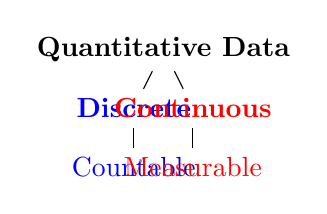
\begin{tikzpicture}[scale=0.5]
	\node {\textbf{Quantitative Data}}
		child {node {\color{blue}\textbf{Discrete}}
			child {node {\color{blue}Countable}}}
		child {node {\color{red}\textbf{Continuous}}
			child {node {\color{red}Measurable}}};
\end{tikzpicture}
\end{center}
\end{frame}

\begin{frame}{Example 2}
Determine whether each quantiative variable is discrete or continuous.	\newline\\	
(a)	\quad Number of free throws made.	\quad	\pause
Discrete \newline\\ \pause
(b) \quad Time it takes to finish a book. \quad \pause
Continuous \newline\\ \pause
(c) \quad Water pressure from a fire hose. \quad \pause
Continuous \newline\\ \pause
(d) \quad The amount of money in a retirement account. \quad \pause Discrete
\end{frame}

\section{Classify data by its level of measurement}

\begin{frame}{Nominal Level of Measurement}
In addition to qualitative and quantitative (and the quantitative variables discrete and continuous), there are 4 different levels of measurement of data.	\newline\\	\pause
\begin{tcolorbox}[colframe=green!20!black, colback = green!30!white,title=\textbf{Nominal Level of Data}]
The \textbf{nominal level of measurement} involves only categorical data; the data can't be arranged in a meaningful order.
\end{tcolorbox}
\end{frame}

\begin{frame}{Ordinal Level of Measurement}
\begin{tcolorbox}[colframe=green!20!black, colback = green!30!white,title=\textbf{Ordinal Level of Data}]
The \textbf{ordinal level of measurement} involves data that can be arranged in a meaningful order, but differences in data values can't be found or are meaningless.
\end{tcolorbox}
\end{frame}

\begin{frame}{Interval Level of Measurement}
\begin{tcolorbox}[colframe=green!20!black, colback = green!30!white,title=\textbf{Interval Level of Data}]
The \textbf{interval level of measurement} involves data that can be arranged in a meaningful order, the differences are meaningful, but ratios are meaningless.
\end{tcolorbox}
\vspace{10pt}	\pause
\emph{Note}: With interval level of measurement, there is no natural zero starting point and negative values can exist.
\end{frame}

\begin{frame}{Ratio Level of Measurement}
\begin{tcolorbox}[colframe=green!20!black, colback = green!30!white,title=\textbf{Ratio Level of Data}]
The \textbf{ratio level of measurement} involves data that can be arranged in a meaningful order, the differences are meaningful, but there is a natural zero starting point and ratios are meaningful.
\end{tcolorbox}
\end{frame}

\begin{frame}{Example 3}
Classify each by level of measurement.	\newline\\
(a) \quad Top 10 cities to live in. 	\quad \pause Ordinal \newline\\ \pause
(b) \quad Amount of coffee in a cup. \quad \pause Ratio \newline\\ \pause
(c) \quad Room temperature (in degrees Celsius). \quad \pause Interval \newline\\ \pause
(d) \quad Your blood type. \quad \pause Nominal
\end{frame}

\end{document}